\documentclass[1p]{elsarticle_modified}
%\bibliographystyle{elsarticle-num}

%\usepackage[colorlinks]{hyperref}
%\usepackage{abbrmath_seonhwa} %\Abb, \Ascr, \Acal ,\Abf, \Afrak
\usepackage{amsfonts}
\usepackage{amssymb}
\usepackage{amsmath}
\usepackage{amsthm}
\usepackage{scalefnt}
\usepackage{amsbsy}
\usepackage{kotex}
\usepackage{caption}
\usepackage{subfig}
\usepackage{color}
\usepackage{graphicx}
\usepackage{xcolor} %% white, black, red, green, blue, cyan, magenta, yellow
\usepackage{float}
\usepackage{setspace}
\usepackage{hyperref}

\usepackage{tikz}
\usetikzlibrary{arrows}

\usepackage{multirow}
\usepackage{array} % fixed length table
\usepackage{hhline}

%%%%%%%%%%%%%%%%%%%%%
\makeatletter
\renewcommand*\env@matrix[1][\arraystretch]{%
	\edef\arraystretch{#1}%
	\hskip -\arraycolsep
	\let\@ifnextchar\new@ifnextchar
	\array{*\c@MaxMatrixCols c}}
\makeatother %https://tex.stackexchange.com/questions/14071/how-can-i-increase-the-line-spacing-in-a-matrix
%%%%%%%%%%%%%%%

\usepackage[normalem]{ulem}

\newcommand{\msout}[1]{\ifmmode\text{\sout{\ensuremath{#1}}}\else\sout{#1}\fi}
%SOURCE: \msout is \stkout macro in https://tex.stackexchange.com/questions/20609/strikeout-in-math-mode

\newcommand{\cancel}[1]{
	\ifmmode
	{\color{red}\msout{#1}}
	\else
	{\color{red}\sout{#1}}
	\fi
}

\newcommand{\add}[1]{
	{\color{blue}\uwave{#1}}
}

\newcommand{\replace}[2]{
	\ifmmode
	{\color{red}\msout{#1}}{\color{blue}\uwave{#2}}
	\else
	{\color{red}\sout{#1}}{\color{blue}\uwave{#2}}
	\fi
}

\newcommand{\Sol}{\mathcal{S}} %segment
\newcommand{\D}{D} %diagram
\newcommand{\A}{\mathcal{A}} %arc


%%%%%%%%%%%%%%%%%%%%%%%%%%%%%5 test

\def\sl{\operatorname{\textup{SL}}(2,\Cbb)}
\def\psl{\operatorname{\textup{PSL}}(2,\Cbb)}
\def\quan{\mkern 1mu \triangleright \mkern 1mu}

\theoremstyle{definition}
\newtheorem{thm}{Theorem}[section]
\newtheorem{prop}[thm]{Proposition}
\newtheorem{lem}[thm]{Lemma}
\newtheorem{ques}[thm]{Question}
\newtheorem{cor}[thm]{Corollary}
\newtheorem{defn}[thm]{Definition}
\newtheorem{exam}[thm]{Example}
\newtheorem{rmk}[thm]{Remark}
\newtheorem{alg}[thm]{Algorithm}

\newcommand{\I}{\sqrt{-1}}
\begin{document}

%\begin{frontmatter}
%
%\title{Boundary parabolic representations of knots up to 8 crossings}
%
%%% Group authors per affiliation:
%\author{Yunhi Cho} 
%\address{Department of Mathematics, University of Seoul, Seoul, Korea}
%\ead{yhcho@uos.ac.kr}
%
%
%\author{Seonhwa Kim} %\fnref{s_kim}}
%\address{Center for Geometry and Physics, Institute for Basic Science, Pohang, 37673, Korea}
%\ead{ryeona17@ibs.re.kr}
%
%\author{Hyuk Kim}
%\address{Department of Mathematical Sciences, Seoul National University, Seoul 08826, Korea}
%\ead{hyukkim@snu.ac.kr}
%
%\author{Seokbeom Yoon}
%\address{Department of Mathematical Sciences, Seoul National University, Seoul, 08826,  Korea}
%\ead{sbyoon15@snu.ac.kr}
%
%\begin{abstract}
%We find all boundary parabolic representation of knots up to 8 crossings.
%
%\end{abstract}
%\begin{keyword}
%    \MSC[2010] 57M25 
%\end{keyword}
%
%\end{frontmatter}

%\linenumbers
%\tableofcontents
%
\newcommand\colored[1]{\textcolor{white}{\rule[-0.35ex]{0.8em}{1.4ex}}\kern-0.8em\color{red} #1}%
%\newcommand\colored[1]{\textcolor{white}{ #1}\kern-2.17ex	\textcolor{white}{ #1}\kern-1.81ex	\textcolor{white}{ #1}\kern-2.15ex\color{red}#1	}

{\Large $\underline{12a_{0271}~(K12a_{0271})}$}

\setlength{\tabcolsep}{10pt}
\renewcommand{\arraystretch}{1.6}
\vspace{1cm}\begin{tabular}{m{100pt}>{\centering\arraybackslash}m{274pt}}
\multirow{5}{120pt}{
	\centering
	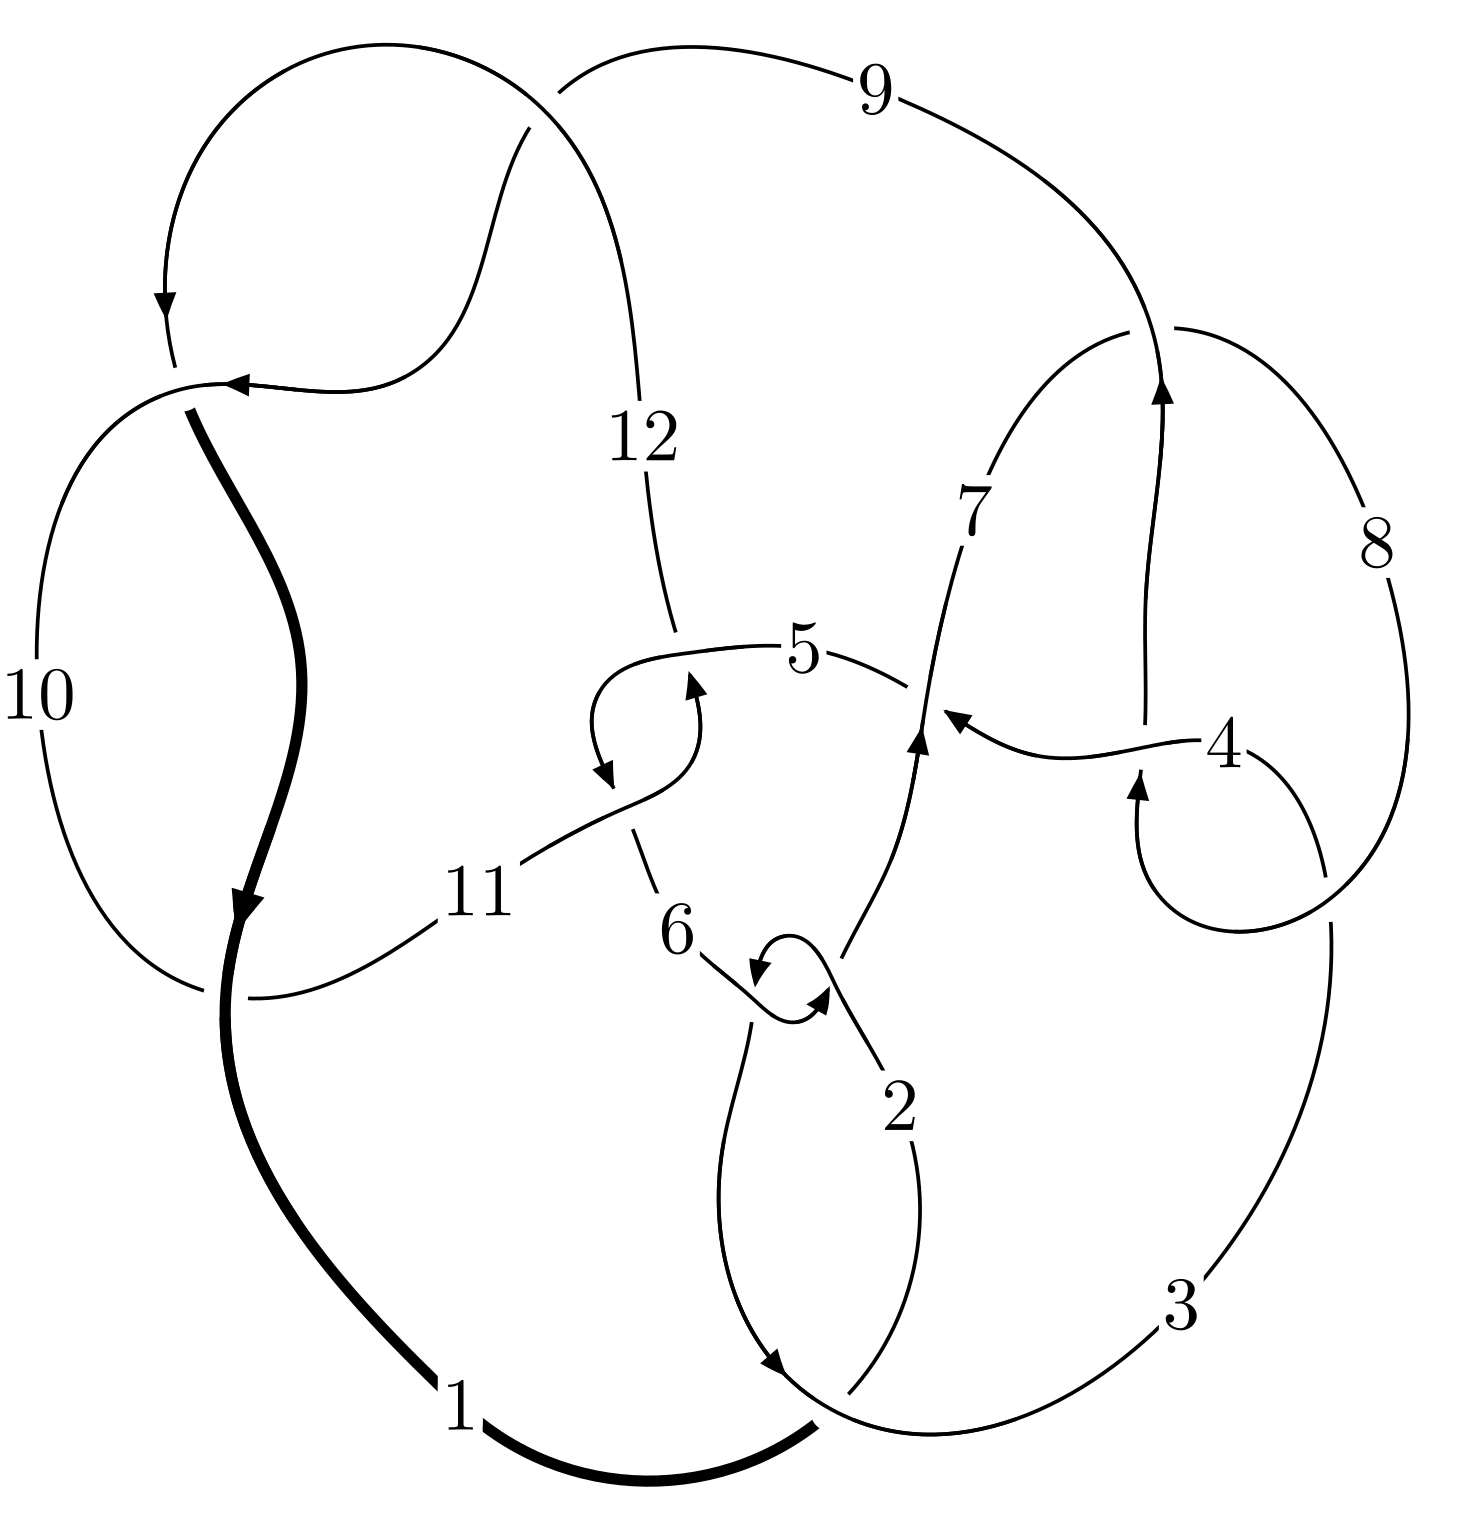
\includegraphics[width=112pt]{../../../GIT/diagram.site/Diagrams/png/1072_12a_0271.png}\\
\ \ \ A knot diagram\footnotemark}&
\allowdisplaybreaks
\textbf{Linearized knot diagam} \\
\cline{2-2}
 &
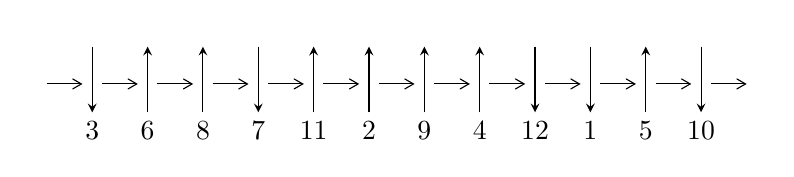
\begin{tikzpicture}[x=20pt, y=17pt]
	% nodes
	\node (C0) at (0, 0) {};
	\node (C1) at (1, 0) {};
	\node (C1U) at (1, +1) {};
	\node (C1D) at (1, -1) {3};

	\node (C2) at (2, 0) {};
	\node (C2U) at (2, +1) {};
	\node (C2D) at (2, -1) {6};

	\node (C3) at (3, 0) {};
	\node (C3U) at (3, +1) {};
	\node (C3D) at (3, -1) {8};

	\node (C4) at (4, 0) {};
	\node (C4U) at (4, +1) {};
	\node (C4D) at (4, -1) {7};

	\node (C5) at (5, 0) {};
	\node (C5U) at (5, +1) {};
	\node (C5D) at (5, -1) {11};

	\node (C6) at (6, 0) {};
	\node (C6U) at (6, +1) {};
	\node (C6D) at (6, -1) {2};

	\node (C7) at (7, 0) {};
	\node (C7U) at (7, +1) {};
	\node (C7D) at (7, -1) {9};

	\node (C8) at (8, 0) {};
	\node (C8U) at (8, +1) {};
	\node (C8D) at (8, -1) {4};

	\node (C9) at (9, 0) {};
	\node (C9U) at (9, +1) {};
	\node (C9D) at (9, -1) {12};

	\node (C10) at (10, 0) {};
	\node (C10U) at (10, +1) {};
	\node (C10D) at (10, -1) {1};

	\node (C11) at (11, 0) {};
	\node (C11U) at (11, +1) {};
	\node (C11D) at (11, -1) {5};

	\node (C12) at (12, 0) {};
	\node (C12U) at (12, +1) {};
	\node (C12D) at (12, -1) {10};
	\node (C13) at (13, 0) {};

	% arrows
	\draw[->,>={angle 60}]
	(C0) edge (C1) (C1) edge (C2) (C2) edge (C3) (C3) edge (C4) (C4) edge (C5) (C5) edge (C6) (C6) edge (C7) (C7) edge (C8) (C8) edge (C9) (C9) edge (C10) (C10) edge (C11) (C11) edge (C12) (C12) edge (C13) ;	\draw[->,>=stealth]
	(C1U) edge (C1D) (C2D) edge (C2U) (C3D) edge (C3U) (C4U) edge (C4D) (C5D) edge (C5U) (C6D) edge (C6U) (C7D) edge (C7U) (C8D) edge (C8U) (C9U) edge (C9D) (C10U) edge (C10D) (C11D) edge (C11U) (C12U) edge (C12D) ;
	\end{tikzpicture} \\
\hhline{~~} \\& 
\textbf{Solving Sequence} \\ \cline{2-2} 
 &
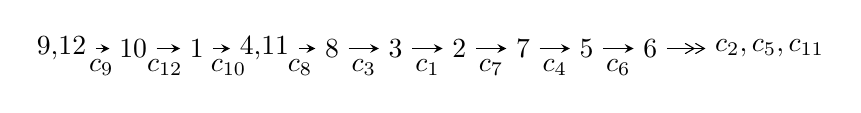
\begin{tikzpicture}[x=23pt, y=7pt]
	% node
	\node (A0) at (-1/8, 0) {9,12};
	\node (A1) at (1, 0) {10};
	\node (A2) at (2, 0) {1};
	\node (A3) at (49/16, 0) {4,11};
	\node (A4) at (33/8, 0) {8};
	\node (A5) at (41/8, 0) {3};
	\node (A6) at (49/8, 0) {2};
	\node (A7) at (57/8, 0) {7};
	\node (A8) at (65/8, 0) {5};
	\node (A9) at (73/8, 0) {6};
	\node (C1) at (1/2, -1) {$c_{9}$};
	\node (C2) at (3/2, -1) {$c_{12}$};
	\node (C3) at (5/2, -1) {$c_{10}$};
	\node (C4) at (29/8, -1) {$c_{8}$};
	\node (C5) at (37/8, -1) {$c_{3}$};
	\node (C6) at (45/8, -1) {$c_{1}$};
	\node (C7) at (53/8, -1) {$c_{7}$};
	\node (C8) at (61/8, -1) {$c_{4}$};
	\node (C9) at (69/8, -1) {$c_{6}$};
	\node (A10) at (11, 0) {$c_{2},c_{5},c_{11}$};

	% edge
	\draw[->,>=stealth]	
	(A0) edge (A1) (A1) edge (A2) (A2) edge (A3) (A3) edge (A4) (A4) edge (A5) (A5) edge (A6) (A6) edge (A7) (A7) edge (A8) (A8) edge (A9) ;
	\draw[->>,>={angle 60}]	
	(A9) edge (A10);
\end{tikzpicture} \\ 

\end{tabular} \\

\footnotetext{
The image of knot diagram is generated by the software ``\textbf{Draw programme}" developed by Andrew Bartholomew(\url{http://www.layer8.co.uk/maths/draw/index.htm\#Running-draw}), where we modified some parts for our purpose(\url{https://github.com/CATsTAILs/LinksPainter}).
}\phantom \\ \newline 
\centering \textbf{Ideals for irreducible components\footnotemark of $X_{\text{par}}$} 
 
\begin{align*}
I^u_{1}&=\langle 
1.23243\times10^{129} u^{108}+1.55838\times10^{130} u^{107}+\cdots+3.15285\times10^{126} b+9.10169\times10^{128},\\
\phantom{I^u_{1}}&\phantom{= \langle  }6.10588\times10^{129} u^{108}+7.74537\times10^{130} u^{107}+\cdots+6.30570\times10^{126} a+4.64339\times10^{129},\\
\phantom{I^u_{1}}&\phantom{= \langle  }u^{109}+14 u^{108}+\cdots+7 u+1\rangle \\
I^u_{2}&=\langle 
23 a^8+230 a^7+849 a^6+1550 a^5+2020 a^4+2255 a^3+1022 a^2+145 b+663 a-205,\\
\phantom{I^u_{2}}&\phantom{= \langle  }a^9+7 a^8+17 a^7+26 a^6+42 a^5+30 a^4+34 a^3+9 a^2+8 a-1,\;u-1\rangle \\
I^u_{3}&=\langle 
-134 a^3 u+33 a^3-58 a^2 u-279 a^2-52 a u+1310 b-476 a+52 u-834,\\
\phantom{I^u_{3}}&\phantom{= \langle  }a^4+2 a^3 u+4 a^3+6 a^2 u+13 a^2+14 a u+22 a+30 u+52,\;u^2+u-1\rangle \\
\\
\end{align*}
\raggedright * 3 irreducible components of $\dim_{\mathbb{C}}=0$, with total 126 representations.\\
\footnotetext{All coefficients of polynomials are rational numbers. But the coefficients are sometimes approximated in decimal forms when there is not enough margin.}
\newpage
\renewcommand{\arraystretch}{1}
\centering \section*{I. $I^u_{1}= \langle 1.23\times10^{129} u^{108}+1.56\times10^{130} u^{107}+\cdots+3.15\times10^{126} b+9.10\times10^{128},\;6.11\times10^{129} u^{108}+7.75\times10^{130} u^{107}+\cdots+6.31\times10^{126} a+4.64\times10^{129},\;u^{109}+14 u^{108}+\cdots+7 u+1 \rangle$}
\flushleft \textbf{(i) Arc colorings}\\
\begin{tabular}{m{7pt} m{180pt} m{7pt} m{180pt} }
\flushright $a_{9}=$&$\begin{pmatrix}1\\0\end{pmatrix}$ \\
\flushright $a_{12}=$&$\begin{pmatrix}0\\u\end{pmatrix}$ \\
\flushright $a_{10}=$&$\begin{pmatrix}1\\u^2\end{pmatrix}$ \\
\flushright $a_{1}=$&$\begin{pmatrix}- u\\- u^3+u\end{pmatrix}$ \\
\flushright $a_{4}=$&$\begin{pmatrix}-968.311 u^{108}-12283.1 u^{107}+\cdots-4584.18 u-736.380\\-390.893 u^{108}-4942.78 u^{107}+\cdots-1804.94 u-288.681\end{pmatrix}$ \\
\flushright $a_{11}=$&$\begin{pmatrix}- u^2+1\\- u^4+2 u^2\end{pmatrix}$ \\
\flushright $a_{8}=$&$\begin{pmatrix}-929.018 u^{108}-11751.3 u^{107}+\cdots-4271.39 u-682.333\\-735.325 u^{108}-9383.18 u^{107}+\cdots-3627.78 u-583.409\end{pmatrix}$ \\
\flushright $a_{3}=$&$\begin{pmatrix}-244.974 u^{108}-3068.45 u^{107}+\cdots-1003.44 u-164.812\\679.242 u^{108}+8687.50 u^{107}+\cdots+3444.28 u+556.251\end{pmatrix}$ \\
\flushright $a_{2}=$&$\begin{pmatrix}328.541 u^{108}+4085.82 u^{107}+\cdots+1244.91 u+200.212\\29.4565 u^{108}+399.793 u^{107}+\cdots+227.612 u+39.0444\end{pmatrix}$ \\
\flushright $a_{7}=$&$\begin{pmatrix}-193.693 u^{108}-2368.15 u^{107}+\cdots-643.610 u-98.9239\\-735.325 u^{108}-9383.18 u^{107}+\cdots-3627.78 u-583.409\end{pmatrix}$ \\
\flushright $a_{5}=$&$\begin{pmatrix}763.605 u^{108}+9680.35 u^{107}+\cdots+3621.10 u+578.034\\-1957.98 u^{108}-24889.9 u^{107}+\cdots-9485.41 u-1525.65\end{pmatrix}$ \\
\flushright $a_{6}=$&$\begin{pmatrix}-13.8716 u^{108}-155.907 u^{107}+\cdots+8.72015 u+0.253671\\-1586.38 u^{108}-20163.0 u^{107}+\cdots-7667.22 u-1232.67\end{pmatrix}$\\&\end{tabular}
\flushleft \textbf{(ii) Obstruction class $= -1$}\\~\\
\flushleft \textbf{(iii) Cusp Shapes $= 1327.30 u^{108}+16843.2 u^{107}+\cdots+6329.93 u+1019.14$}\\~\\
\newpage\renewcommand{\arraystretch}{1}
\flushleft \textbf{(iv) u-Polynomials at the component}\newline \\
\begin{tabular}{m{50pt}|m{274pt}}
Crossings & \hspace{64pt}u-Polynomials at each crossing \\
\hline $$\begin{aligned}c_{1}\end{aligned}$$&$\begin{aligned}
&u^{109}+56 u^{108}+\cdots-5688 u-1296
\end{aligned}$\\
\hline $$\begin{aligned}c_{2},c_{6}\end{aligned}$$&$\begin{aligned}
&u^{109}-2 u^{108}+\cdots+72 u-36
\end{aligned}$\\
\hline $$\begin{aligned}c_{3},c_{8}\end{aligned}$$&$\begin{aligned}
&u^{109}-2 u^{108}+\cdots+15 u-9
\end{aligned}$\\
\hline $$\begin{aligned}c_{4}\end{aligned}$$&$\begin{aligned}
&u^{109}-6 u^{108}+\cdots+1068687 u-322299
\end{aligned}$\\
\hline $$\begin{aligned}c_{5},c_{11}\end{aligned}$$&$\begin{aligned}
&u^{109}+u^{108}+\cdots-6144 u-512
\end{aligned}$\\
\hline $$\begin{aligned}c_{7}\end{aligned}$$&$\begin{aligned}
&u^{109}-52 u^{108}+\cdots-189 u-81
\end{aligned}$\\
\hline $$\begin{aligned}c_{9},c_{10},c_{12}\end{aligned}$$&$\begin{aligned}
&u^{109}-14 u^{108}+\cdots+7 u-1
\end{aligned}$\\
\hline
\end{tabular}\\~\\
\newpage\renewcommand{\arraystretch}{1}
\flushleft \textbf{(v) Riley Polynomials at the component}\newline \\
\begin{tabular}{m{50pt}|m{274pt}}
Crossings & \hspace{64pt}Riley Polynomials at each crossing \\
\hline $$\begin{aligned}c_{1}\end{aligned}$$&$\begin{aligned}
&y^{109}+4 y^{108}+\cdots+86720544 y-1679616
\end{aligned}$\\
\hline $$\begin{aligned}c_{2},c_{6}\end{aligned}$$&$\begin{aligned}
&y^{109}+56 y^{108}+\cdots-5688 y-1296
\end{aligned}$\\
\hline $$\begin{aligned}c_{3},c_{8}\end{aligned}$$&$\begin{aligned}
&y^{109}-52 y^{108}+\cdots-189 y-81
\end{aligned}$\\
\hline $$\begin{aligned}c_{4}\end{aligned}$$&$\begin{aligned}
&y^{109}+20 y^{108}+\cdots-3429890229501 y-103876645401
\end{aligned}$\\
\hline $$\begin{aligned}c_{5},c_{11}\end{aligned}$$&$\begin{aligned}
&y^{109}+69 y^{108}+\cdots+11272192 y-262144
\end{aligned}$\\
\hline $$\begin{aligned}c_{7}\end{aligned}$$&$\begin{aligned}
&y^{109}+16 y^{108}+\cdots+363123 y-6561
\end{aligned}$\\
\hline $$\begin{aligned}c_{9},c_{10},c_{12}\end{aligned}$$&$\begin{aligned}
&y^{109}-108 y^{108}+\cdots+63 y-1
\end{aligned}$\\
\hline
\end{tabular}\\~\\
\newpage\flushleft \textbf{(vi) Complex Volumes and Cusp Shapes}
$$\begin{array}{c|c|c}  
\text{Solutions to }I^u_{1}& \I (\text{vol} + \sqrt{-1}CS) & \text{Cusp shape}\\
 \hline 
\begin{aligned}
u &= \phantom{-}1.016630 + 0.004269 I \\
a &= \phantom{-}8.13325 + 5.59186 I \\
b &= \phantom{-}0.837596 - 0.489489 I\end{aligned}
 & -3.33980 - 2.03615 I & \phantom{-0.000000 } 0 \\ \hline\begin{aligned}
u &= \phantom{-}1.016630 - 0.004269 I \\
a &= \phantom{-}8.13325 - 5.59186 I \\
b &= \phantom{-}0.837596 + 0.489489 I\end{aligned}
 & -3.33980 + 2.03615 I & \phantom{-0.000000 } 0 \\ \hline\begin{aligned}
u &= \phantom{-}0.404790 + 0.937368 I \\
a &= -0.90874 - 1.47581 I \\
b &= \phantom{-}1.124360 - 0.589303 I\end{aligned}
 & -0.76763 - 12.89190 I & \phantom{-0.000000 } 0 \\ \hline\begin{aligned}
u &= \phantom{-}0.404790 - 0.937368 I \\
a &= -0.90874 + 1.47581 I \\
b &= \phantom{-}1.124360 + 0.589303 I\end{aligned}
 & -0.76763 + 12.89190 I & \phantom{-0.000000 } 0 \\ \hline\begin{aligned}
u &= \phantom{-}0.411108 + 0.884965 I \\
a &= \phantom{-}0.521196 + 0.355803 I \\
b &= \phantom{-}0.369946 + 0.793260 I\end{aligned}
 & -3.00544 - 7.70749 I & \phantom{-0.000000 } 0 \\ \hline\begin{aligned}
u &= \phantom{-}0.411108 - 0.884965 I \\
a &= \phantom{-}0.521196 - 0.355803 I \\
b &= \phantom{-}0.369946 - 0.793260 I\end{aligned}
 & -3.00544 + 7.70749 I & \phantom{-0.000000 } 0 \\ \hline\begin{aligned}
u &= \phantom{-}1.016580 + 0.274813 I \\
a &= \phantom{-}0.484768 + 0.857560 I \\
b &= \phantom{-}0.012958 + 0.405942 I\end{aligned}
 & -1.93065 - 0.92430 I & \phantom{-0.000000 } 0 \\ \hline\begin{aligned}
u &= \phantom{-}1.016580 - 0.274813 I \\
a &= \phantom{-}0.484768 - 0.857560 I \\
b &= \phantom{-}0.012958 - 0.405942 I\end{aligned}
 & -1.93065 + 0.92430 I & \phantom{-0.000000 } 0 \\ \hline\begin{aligned}
u &= \phantom{-}0.786470 + 0.711560 I \\
a &= -0.139650 - 0.997227 I \\
b &= \phantom{-}0.385614 - 0.697857 I\end{aligned}
 & -4.16608 + 2.27907 I & \phantom{-0.000000 } 0 \\ \hline\begin{aligned}
u &= \phantom{-}0.786470 - 0.711560 I \\
a &= -0.139650 + 0.997227 I \\
b &= \phantom{-}0.385614 + 0.697857 I\end{aligned}
 & -4.16608 - 2.27907 I & \phantom{-0.000000 } 0\\
 \hline 
 \end{array}$$\newpage$$\begin{array}{c|c|c}  
\text{Solutions to }I^u_{1}& \I (\text{vol} + \sqrt{-1}CS) & \text{Cusp shape}\\
 \hline 
\begin{aligned}
u &= \phantom{-}0.912194 + 0.564468 I \\
a &= \phantom{-}0.124511 - 0.334015 I \\
b &= -1.052250 - 0.499335 I\end{aligned}
 & \phantom{-}0.05579 + 2.65712 I & \phantom{-0.000000 } 0 \\ \hline\begin{aligned}
u &= \phantom{-}0.912194 - 0.564468 I \\
a &= \phantom{-}0.124511 + 0.334015 I \\
b &= -1.052250 + 0.499335 I\end{aligned}
 & \phantom{-}0.05579 - 2.65712 I & \phantom{-0.000000 } 0 \\ \hline\begin{aligned}
u &= \phantom{-}0.320133 + 0.851289 I \\
a &= \phantom{-}1.19396 + 1.23612 I \\
b &= -1.114450 + 0.552127 I\end{aligned}
 & \phantom{-}1.84711 - 7.63939 I & \phantom{-0.000000 } 0 \\ \hline\begin{aligned}
u &= \phantom{-}0.320133 - 0.851289 I \\
a &= \phantom{-}1.19396 - 1.23612 I \\
b &= -1.114450 - 0.552127 I\end{aligned}
 & \phantom{-}1.84711 + 7.63939 I & \phantom{-0.000000 } 0 \\ \hline\begin{aligned}
u &= \phantom{-}0.301149 + 0.854421 I \\
a &= \phantom{-}1.006620 + 0.099668 I \\
b &= -1.140280 - 0.181677 I\end{aligned}
 & \phantom{-}1.90970 - 5.11227 I & \phantom{-0.000000 } 0 \\ \hline\begin{aligned}
u &= \phantom{-}0.301149 - 0.854421 I \\
a &= \phantom{-}1.006620 - 0.099668 I \\
b &= -1.140280 + 0.181677 I\end{aligned}
 & \phantom{-}1.90970 + 5.11227 I & \phantom{-0.000000 } 0 \\ \hline\begin{aligned}
u &= \phantom{-}0.943762 + 0.586540 I \\
a &= \phantom{-}0.532799 + 1.247840 I \\
b &= -1.044820 + 0.255463 I\end{aligned}
 & -0.0247817 + 0.0796703 I & \phantom{-0.000000 } 0 \\ \hline\begin{aligned}
u &= \phantom{-}0.943762 - 0.586540 I \\
a &= \phantom{-}0.532799 - 1.247840 I \\
b &= -1.044820 - 0.255463 I\end{aligned}
 & -0.0247817 - 0.0796703 I & \phantom{-0.000000 } 0 \\ \hline\begin{aligned}
u &= \phantom{-}0.849998 + 0.764802 I \\
a &= -0.009634 + 0.635203 I \\
b &= \phantom{-}1.093690 + 0.562163 I\end{aligned}
 & -2.10039 + 7.13248 I & \phantom{-0.000000 } 0 \\ \hline\begin{aligned}
u &= \phantom{-}0.849998 - 0.764802 I \\
a &= -0.009634 - 0.635203 I \\
b &= \phantom{-}1.093690 - 0.562163 I\end{aligned}
 & -2.10039 - 7.13248 I & \phantom{-0.000000 } 0\\
 \hline 
 \end{array}$$\newpage$$\begin{array}{c|c|c}  
\text{Solutions to }I^u_{1}& \I (\text{vol} + \sqrt{-1}CS) & \text{Cusp shape}\\
 \hline 
\begin{aligned}
u &= \phantom{-}0.567153 + 0.640929 I \\
a &= \phantom{-}1.006030 - 0.275954 I \\
b &= \phantom{-}0.493383 + 0.632986 I\end{aligned}
 & -4.68801 + 0.41176 I & \phantom{-0.000000 } 0 \\ \hline\begin{aligned}
u &= \phantom{-}0.567153 - 0.640929 I \\
a &= \phantom{-}1.006030 + 0.275954 I \\
b &= \phantom{-}0.493383 - 0.632986 I\end{aligned}
 & -4.68801 - 0.41176 I & \phantom{-0.000000 } 0 \\ \hline\begin{aligned}
u &= \phantom{-}0.454957 + 0.721916 I \\
a &= \phantom{-}0.137567 - 0.733744 I \\
b &= \phantom{-}0.611030 - 0.716852 I\end{aligned}
 & -4.29347 - 5.01697 I & \phantom{-0.000000 } 0 \\ \hline\begin{aligned}
u &= \phantom{-}0.454957 - 0.721916 I \\
a &= \phantom{-}0.137567 + 0.733744 I \\
b &= \phantom{-}0.611030 + 0.716852 I\end{aligned}
 & -4.29347 + 5.01697 I & \phantom{-0.000000 } 0 \\ \hline\begin{aligned}
u &= \phantom{-}0.345213 + 0.752658 I \\
a &= -0.349887 - 0.087687 I \\
b &= -0.320749 - 0.709497 I\end{aligned}
 & -0.44649 - 2.81276 I & \phantom{-0.000000 } 0 \\ \hline\begin{aligned}
u &= \phantom{-}0.345213 - 0.752658 I \\
a &= -0.349887 + 0.087687 I \\
b &= -0.320749 + 0.709497 I\end{aligned}
 & -0.44649 + 2.81276 I & \phantom{-0.000000 } 0 \\ \hline\begin{aligned}
u &= \phantom{-}0.623603 + 0.494487 I \\
a &= \phantom{-}0.307659 + 0.731604 I \\
b &= -0.554457 + 0.508718 I\end{aligned}
 & -1.54674 - 1.43755 I & \phantom{-0.000000 } 0 \\ \hline\begin{aligned}
u &= \phantom{-}0.623603 - 0.494487 I \\
a &= \phantom{-}0.307659 - 0.731604 I \\
b &= -0.554457 - 0.508718 I\end{aligned}
 & -1.54674 + 1.43755 I & \phantom{-0.000000 } 0 \\ \hline\begin{aligned}
u &= \phantom{-}0.428746 + 0.651403 I \\
a &= -2.05459 - 1.82233 I \\
b &= \phantom{-}1.042280 - 0.549995 I\end{aligned}
 & -3.06677 - 4.24362 I & \phantom{-0.000000 } 0 \\ \hline\begin{aligned}
u &= \phantom{-}0.428746 - 0.651403 I \\
a &= -2.05459 + 1.82233 I \\
b &= \phantom{-}1.042280 + 0.549995 I\end{aligned}
 & -3.06677 + 4.24362 I & \phantom{-0.000000 } 0\\
 \hline 
 \end{array}$$\newpage$$\begin{array}{c|c|c}  
\text{Solutions to }I^u_{1}& \I (\text{vol} + \sqrt{-1}CS) & \text{Cusp shape}\\
 \hline 
\begin{aligned}
u &= \phantom{-}1.142100 + 0.435495 I \\
a &= -0.41213 - 1.72843 I \\
b &= \phantom{-}1.064570 - 0.391803 I\end{aligned}
 & \phantom{-}0.71816 - 4.11005 I & \phantom{-0.000000 } 0 \\ \hline\begin{aligned}
u &= \phantom{-}1.142100 - 0.435495 I \\
a &= -0.41213 + 1.72843 I \\
b &= \phantom{-}1.064570 + 0.391803 I\end{aligned}
 & \phantom{-}0.71816 + 4.11005 I & \phantom{-0.000000 } 0 \\ \hline\begin{aligned}
u &= \phantom{-}0.463780 + 0.617736 I \\
a &= -0.527069 + 1.057310 I \\
b &= \phantom{-}0.976057 + 0.625465 I\end{aligned}
 & -3.21393 + 0.11148 I & \phantom{-0.000000 } 0 \\ \hline\begin{aligned}
u &= \phantom{-}0.463780 - 0.617736 I \\
a &= -0.527069 - 1.057310 I \\
b &= \phantom{-}0.976057 - 0.625465 I\end{aligned}
 & -3.21393 - 0.11148 I & \phantom{-0.000000 } 0 \\ \hline\begin{aligned}
u &= -1.249550 + 0.003143 I \\
a &= -0.283939 + 0.688479 I \\
b &= \phantom{-}1.234130 + 0.398669 I\end{aligned}
 & \phantom{-}1.78465 + 1.35351 I & \phantom{-0.000000 } 0 \\ \hline\begin{aligned}
u &= -1.249550 - 0.003143 I \\
a &= -0.283939 - 0.688479 I \\
b &= \phantom{-}1.234130 - 0.398669 I\end{aligned}
 & \phantom{-}1.78465 - 1.35351 I & \phantom{-0.000000 } 0 \\ \hline\begin{aligned}
u &= \phantom{-}1.206400 + 0.327884 I \\
a &= -0.389297 + 0.143393 I \\
b &= -1.037800 - 0.324158 I\end{aligned}
 & \phantom{-}0.50722 + 1.42907 I & \phantom{-0.000000 } 0 \\ \hline\begin{aligned}
u &= \phantom{-}1.206400 - 0.327884 I \\
a &= -0.389297 - 0.143393 I \\
b &= -1.037800 + 0.324158 I\end{aligned}
 & \phantom{-}0.50722 - 1.42907 I & \phantom{-0.000000 } 0 \\ \hline\begin{aligned}
u &= \phantom{-}0.148361 + 0.734114 I \\
a &= -1.44030 + 0.28159 I \\
b &= \phantom{-}1.111060 + 0.271317 I\end{aligned}
 & \phantom{-}3.73455 - 0.07956 I & \phantom{-0.000000 } 0 \\ \hline\begin{aligned}
u &= \phantom{-}0.148361 - 0.734114 I \\
a &= -1.44030 - 0.28159 I \\
b &= \phantom{-}1.111060 - 0.271317 I\end{aligned}
 & \phantom{-}3.73455 + 0.07956 I & \phantom{-0.000000 } 0\\
 \hline 
 \end{array}$$\newpage$$\begin{array}{c|c|c}  
\text{Solutions to }I^u_{1}& \I (\text{vol} + \sqrt{-1}CS) & \text{Cusp shape}\\
 \hline 
\begin{aligned}
u &= -1.251330 + 0.110567 I \\
a &= \phantom{-}0.310557 - 1.114140 I \\
b &= -1.219260 - 0.473681 I\end{aligned}
 & \phantom{-}1.25854 + 7.78889 I & \phantom{-0.000000 } 0 \\ \hline\begin{aligned}
u &= -1.251330 - 0.110567 I \\
a &= \phantom{-}0.310557 + 1.114140 I \\
b &= -1.219260 + 0.473681 I\end{aligned}
 & \phantom{-}1.25854 - 7.78889 I & \phantom{-0.000000 } 0 \\ \hline\begin{aligned}
u &= -1.295240 + 0.056218 I \\
a &= -0.164026 + 0.829289 I \\
b &= -0.067094 + 0.861154 I\end{aligned}
 & -2.25141 + 3.00990 I & \phantom{-0.000000 } 0 \\ \hline\begin{aligned}
u &= -1.295240 - 0.056218 I \\
a &= -0.164026 - 0.829289 I \\
b &= -0.067094 - 0.861154 I\end{aligned}
 & -2.25141 - 3.00990 I & \phantom{-0.000000 } 0 \\ \hline\begin{aligned}
u &= -0.082194 + 0.675232 I \\
a &= \phantom{-}0.899320 - 0.233825 I \\
b &= -1.134390 + 0.407127 I\end{aligned}
 & \phantom{-}4.49085 - 5.11092 I & \phantom{-0.000000 } 0 \\ \hline\begin{aligned}
u &= -0.082194 - 0.675232 I \\
a &= \phantom{-}0.899320 + 0.233825 I \\
b &= -1.134390 - 0.407127 I\end{aligned}
 & \phantom{-}4.49085 + 5.11092 I & \phantom{-0.000000 } 0 \\ \hline\begin{aligned}
u &= \phantom{-}1.325510 + 0.015098 I \\
a &= -0.68029 + 2.85029 I \\
b &= -1.011680 + 0.589449 I\end{aligned}
 & -5.19776 - 2.18585 I & \phantom{-0.000000 } 0 \\ \hline\begin{aligned}
u &= \phantom{-}1.325510 - 0.015098 I \\
a &= -0.68029 - 2.85029 I \\
b &= -1.011680 - 0.589449 I\end{aligned}
 & -5.19776 + 2.18585 I & \phantom{-0.000000 } 0 \\ \hline\begin{aligned}
u &= \phantom{-}1.329390 + 0.112204 I \\
a &= \phantom{-}1.13368 + 1.20869 I \\
b &= \phantom{-}0.402859 + 0.628401 I\end{aligned}
 & -3.01364 - 0.75193 I & \phantom{-0.000000 } 0 \\ \hline\begin{aligned}
u &= \phantom{-}1.329390 - 0.112204 I \\
a &= \phantom{-}1.13368 - 1.20869 I \\
b &= \phantom{-}0.402859 - 0.628401 I\end{aligned}
 & -3.01364 + 0.75193 I & \phantom{-0.000000 } 0\\
 \hline 
 \end{array}$$\newpage$$\begin{array}{c|c|c}  
\text{Solutions to }I^u_{1}& \I (\text{vol} + \sqrt{-1}CS) & \text{Cusp shape}\\
 \hline 
\begin{aligned}
u &= \phantom{-}1.373420 + 0.042297 I \\
a &= -1.41682 + 1.56257 I \\
b &= -0.553024 + 0.689823 I\end{aligned}
 & -6.55401 - 2.75061 I & \phantom{-0.000000 } 0 \\ \hline\begin{aligned}
u &= \phantom{-}1.373420 - 0.042297 I \\
a &= -1.41682 - 1.56257 I \\
b &= -0.553024 - 0.689823 I\end{aligned}
 & -6.55401 + 2.75061 I & \phantom{-0.000000 } 0 \\ \hline\begin{aligned}
u &= -0.460518 + 0.401129 I \\
a &= \phantom{-}0.33891 - 2.30443 I \\
b &= -1.140320 - 0.523300 I\end{aligned}
 & \phantom{-}2.81375 + 7.97265 I & \phantom{-}6.75785 - 7.76688 I \\ \hline\begin{aligned}
u &= -0.460518 - 0.401129 I \\
a &= \phantom{-}0.33891 + 2.30443 I \\
b &= -1.140320 + 0.523300 I\end{aligned}
 & \phantom{-}2.81375 - 7.97265 I & \phantom{-}6.75785 + 7.76688 I \\ \hline\begin{aligned}
u &= \phantom{-}1.383490 + 0.198811 I \\
a &= \phantom{-}0.27751 - 2.31980 I \\
b &= \phantom{-}1.078330 - 0.543261 I\end{aligned}
 & -1.04938 - 5.38156 I & \phantom{-0.000000 } 0 \\ \hline\begin{aligned}
u &= \phantom{-}1.383490 - 0.198811 I \\
a &= \phantom{-}0.27751 + 2.31980 I \\
b &= \phantom{-}1.078330 + 0.543261 I\end{aligned}
 & -1.04938 + 5.38156 I & \phantom{-0.000000 } 0 \\ \hline\begin{aligned}
u &= \phantom{-}1.380860 + 0.221289 I \\
a &= \phantom{-}0.651853 - 0.050411 I \\
b &= \phantom{-}1.079270 + 0.187980 I\end{aligned}
 & -1.05843 - 2.88175 I & \phantom{-0.000000 } 0 \\ \hline\begin{aligned}
u &= \phantom{-}1.380860 - 0.221289 I \\
a &= \phantom{-}0.651853 + 0.050411 I \\
b &= \phantom{-}1.079270 - 0.187980 I\end{aligned}
 & -1.05843 + 2.88175 I & \phantom{-0.000000 } 0 \\ \hline\begin{aligned}
u &= -0.270752 + 0.530344 I \\
a &= -0.257115 + 0.691543 I \\
b &= \phantom{-}1.134540 - 0.317097 I\end{aligned}
 & \phantom{-}4.20308 + 0.05931 I & \phantom{-}8.59381 + 0. I\phantom{ +0.000000I} \\ \hline\begin{aligned}
u &= -0.270752 - 0.530344 I \\
a &= -0.257115 - 0.691543 I \\
b &= \phantom{-}1.134540 + 0.317097 I\end{aligned}
 & \phantom{-}4.20308 - 0.05931 I & \phantom{-}8.59381 + 0. I\phantom{ +0.000000I}\\
 \hline 
 \end{array}$$\newpage$$\begin{array}{c|c|c}  
\text{Solutions to }I^u_{1}& \I (\text{vol} + \sqrt{-1}CS) & \text{Cusp shape}\\
 \hline 
\begin{aligned}
u &= -1.380480 + 0.266205 I \\
a &= -0.080388 + 0.259982 I \\
b &= \phantom{-}1.200820 - 0.191115 I\end{aligned}
 & -1.15287 + 3.63290 I & \phantom{-0.000000 } 0 \\ \hline\begin{aligned}
u &= -1.380480 - 0.266205 I \\
a &= -0.080388 - 0.259982 I \\
b &= \phantom{-}1.200820 + 0.191115 I\end{aligned}
 & -1.15287 - 3.63290 I & \phantom{-0.000000 } 0 \\ \hline\begin{aligned}
u &= -0.267350 + 0.518380 I \\
a &= -1.09999 + 2.03371 I \\
b &= \phantom{-}1.126850 + 0.452815 I\end{aligned}
 & \phantom{-}4.19677 + 2.70080 I & \phantom{-}8.69742 - 1.85620 I \\ \hline\begin{aligned}
u &= -0.267350 - 0.518380 I \\
a &= -1.09999 - 2.03371 I \\
b &= \phantom{-}1.126850 - 0.452815 I\end{aligned}
 & \phantom{-}4.19677 - 2.70080 I & \phantom{-}8.69742 + 1.85620 I \\ \hline\begin{aligned}
u &= -1.42886 + 0.12570 I \\
a &= \phantom{-}0.624904 - 0.307615 I \\
b &= -1.108450 + 0.263345 I\end{aligned}
 & -7.14836 - 0.04349 I & \phantom{-0.000000 } 0 \\ \hline\begin{aligned}
u &= -1.42886 - 0.12570 I \\
a &= \phantom{-}0.624904 + 0.307615 I \\
b &= -1.108450 - 0.263345 I\end{aligned}
 & -7.14836 + 0.04349 I & \phantom{-0.000000 } 0 \\ \hline\begin{aligned}
u &= -1.45766 + 0.09362 I \\
a &= -0.66552 + 1.42703 I \\
b &= -0.918640 + 0.694553 I\end{aligned}
 & -7.56134 - 1.77744 I & \phantom{-0.000000 } 0 \\ \hline\begin{aligned}
u &= -1.45766 - 0.09362 I \\
a &= -0.66552 - 1.42703 I \\
b &= -0.918640 - 0.694553 I\end{aligned}
 & -7.56134 + 1.77744 I & \phantom{-0.000000 } 0 \\ \hline\begin{aligned}
u &= \phantom{-}1.45706 + 0.14043 I \\
a &= -0.99668 - 1.44033 I \\
b &= -0.389827 - 0.753821 I\end{aligned}
 & -5.72245 - 5.15147 I & \phantom{-0.000000 } 0 \\ \hline\begin{aligned}
u &= \phantom{-}1.45706 - 0.14043 I \\
a &= -0.99668 + 1.44033 I \\
b &= -0.389827 + 0.753821 I\end{aligned}
 & -5.72245 + 5.15147 I & \phantom{-0.000000 } 0\\
 \hline 
 \end{array}$$\newpage$$\begin{array}{c|c|c}  
\text{Solutions to }I^u_{1}& \I (\text{vol} + \sqrt{-1}CS) & \text{Cusp shape}\\
 \hline 
\begin{aligned}
u &= -1.47452 + 0.15767 I \\
a &= -0.49541 - 1.54608 I \\
b &= -0.693140 - 0.745975 I\end{aligned}
 & -8.21597 + 3.64315 I & \phantom{-0.000000 } 0 \\ \hline\begin{aligned}
u &= -1.47452 - 0.15767 I \\
a &= -0.49541 + 1.54608 I \\
b &= -0.693140 + 0.745975 I\end{aligned}
 & -8.21597 - 3.64315 I & \phantom{-0.000000 } 0 \\ \hline\begin{aligned}
u &= -1.44827 + 0.33097 I \\
a &= -0.053983 - 0.394503 I \\
b &= -1.207320 + 0.135353 I\end{aligned}
 & -3.69746 + 9.38157 I & \phantom{-0.000000 } 0 \\ \hline\begin{aligned}
u &= -1.44827 - 0.33097 I \\
a &= -0.053983 + 0.394503 I \\
b &= -1.207320 - 0.135353 I\end{aligned}
 & -3.69746 - 9.38157 I & \phantom{-0.000000 } 0 \\ \hline\begin{aligned}
u &= -1.45770 + 0.28932 I \\
a &= -0.893306 + 0.858668 I \\
b &= -0.342996 + 0.833291 I\end{aligned}
 & -6.25498 + 6.61355 I & \phantom{-0.000000 } 0 \\ \hline\begin{aligned}
u &= -1.45770 - 0.28932 I \\
a &= -0.893306 - 0.858668 I \\
b &= -0.342996 - 0.833291 I\end{aligned}
 & -6.25498 - 6.61355 I & \phantom{-0.000000 } 0 \\ \hline\begin{aligned}
u &= -1.47125 + 0.23991 I \\
a &= -0.61335 + 2.09178 I \\
b &= \phantom{-}1.115140 + 0.563775 I\end{aligned}
 & -9.20098 + 7.51308 I & \phantom{-0.000000 } 0 \\ \hline\begin{aligned}
u &= -1.47125 - 0.23991 I \\
a &= -0.61335 - 2.09178 I \\
b &= \phantom{-}1.115140 - 0.563775 I\end{aligned}
 & -9.20098 - 7.51308 I & \phantom{-0.000000 } 0 \\ \hline\begin{aligned}
u &= -1.47703 + 0.22116 I \\
a &= \phantom{-}0.73960 - 1.38654 I \\
b &= \phantom{-}1.001020 - 0.698022 I\end{aligned}
 & -9.48577 + 2.96099 I & \phantom{-0.000000 } 0 \\ \hline\begin{aligned}
u &= -1.47703 - 0.22116 I \\
a &= \phantom{-}0.73960 + 1.38654 I \\
b &= \phantom{-}1.001020 + 0.698022 I\end{aligned}
 & -9.48577 - 2.96099 I & \phantom{-0.000000 } 0\\
 \hline 
 \end{array}$$\newpage$$\begin{array}{c|c|c}  
\text{Solutions to }I^u_{1}& \I (\text{vol} + \sqrt{-1}CS) & \text{Cusp shape}\\
 \hline 
\begin{aligned}
u &= -1.45794 + 0.33062 I \\
a &= \phantom{-}0.27434 - 2.04142 I \\
b &= -1.145410 - 0.593691 I\end{aligned}
 & -3.86036 + 11.90930 I & \phantom{-0.000000 } 0 \\ \hline\begin{aligned}
u &= -1.45794 - 0.33062 I \\
a &= \phantom{-}0.27434 + 2.04142 I \\
b &= -1.145410 + 0.593691 I\end{aligned}
 & -3.86036 - 11.90930 I & \phantom{-0.000000 } 0 \\ \hline\begin{aligned}
u &= \phantom{-}1.49360 + 0.16926 I \\
a &= -0.51766 + 2.19626 I \\
b &= -1.105820 + 0.581728 I\end{aligned}
 & -3.61148 - 10.21280 I & \phantom{-0.000000 } 0 \\ \hline\begin{aligned}
u &= \phantom{-}1.49360 - 0.16926 I \\
a &= -0.51766 - 2.19626 I \\
b &= -1.105820 - 0.581728 I\end{aligned}
 & -3.61148 + 10.21280 I & \phantom{-0.000000 } 0 \\ \hline\begin{aligned}
u &= -0.078882 + 0.490309 I \\
a &= \phantom{-}0.817776 - 0.190481 I \\
b &= \phantom{-}0.033791 - 0.647762 I\end{aligned}
 & \phantom{-}1.23015 - 1.32761 I & \phantom{-}4.63192 + 3.39563 I \\ \hline\begin{aligned}
u &= -0.078882 - 0.490309 I \\
a &= \phantom{-}0.817776 + 0.190481 I \\
b &= \phantom{-}0.033791 + 0.647762 I\end{aligned}
 & \phantom{-}1.23015 + 1.32761 I & \phantom{-}4.63192 - 3.39563 I \\ \hline\begin{aligned}
u &= -0.345451 + 0.355207 I \\
a &= -1.20883 + 0.84661 I \\
b &= -0.235515 + 0.725816 I\end{aligned}
 & \phantom{-}0.19256 + 3.25530 I & \phantom{-}3.54040 - 3.77477 I \\ \hline\begin{aligned}
u &= -0.345451 - 0.355207 I \\
a &= -1.20883 - 0.84661 I \\
b &= -0.235515 - 0.725816 I\end{aligned}
 & \phantom{-}0.19256 - 3.25530 I & \phantom{-}3.54040 + 3.77477 I \\ \hline\begin{aligned}
u &= -1.48934 + 0.25765 I \\
a &= \phantom{-}0.45244 + 1.60841 I \\
b &= \phantom{-}0.630174 + 0.807266 I\end{aligned}
 & -10.59110 + 8.58055 I & \phantom{-0.000000 } 0 \\ \hline\begin{aligned}
u &= -1.48934 - 0.25765 I \\
a &= \phantom{-}0.45244 - 1.60841 I \\
b &= \phantom{-}0.630174 - 0.807266 I\end{aligned}
 & -10.59110 - 8.58055 I & \phantom{-0.000000 } 0\\
 \hline 
 \end{array}$$\newpage$$\begin{array}{c|c|c}  
\text{Solutions to }I^u_{1}& \I (\text{vol} + \sqrt{-1}CS) & \text{Cusp shape}\\
 \hline 
\begin{aligned}
u &= -1.50605 + 0.20053 I \\
a &= \phantom{-}0.971598 - 0.547193 I \\
b &= \phantom{-}0.346235 - 0.727850 I\end{aligned}
 & -11.44530 + 2.58672 I & \phantom{-0.000000 } 0 \\ \hline\begin{aligned}
u &= -1.50605 - 0.20053 I \\
a &= \phantom{-}0.971598 + 0.547193 I \\
b &= \phantom{-}0.346235 + 0.727850 I\end{aligned}
 & -11.44530 - 2.58672 I & \phantom{-0.000000 } 0 \\ \hline\begin{aligned}
u &= -1.50267 + 0.33676 I \\
a &= \phantom{-}0.998701 - 0.957933 I \\
b &= \phantom{-}0.389482 - 0.855808 I\end{aligned}
 & -9.1719 + 12.1476 I & \phantom{-0.000000 } 0 \\ \hline\begin{aligned}
u &= -1.50267 - 0.33676 I \\
a &= \phantom{-}0.998701 + 0.957933 I \\
b &= \phantom{-}0.389482 + 0.855808 I\end{aligned}
 & -9.1719 - 12.1476 I & \phantom{-0.000000 } 0 \\ \hline\begin{aligned}
u &= -1.50887 + 0.36177 I \\
a &= -0.15566 + 2.15597 I \\
b &= \phantom{-}1.139470 + 0.617419 I\end{aligned}
 & -6.9159 + 17.6040 I & \phantom{-0.000000 } 0 \\ \hline\begin{aligned}
u &= -1.50887 - 0.36177 I \\
a &= -0.15566 - 2.15597 I \\
b &= \phantom{-}1.139470 - 0.617419 I\end{aligned}
 & -6.9159 - 17.6040 I & \phantom{-0.000000 } 0 \\ \hline\begin{aligned}
u &= -1.61741 + 0.14592 I \\
a &= \phantom{-}0.36078 + 1.47913 I \\
b &= \phantom{-}0.539268 + 0.620370 I\end{aligned}
 & -12.38970 + 0.73229 I & \phantom{-0.000000 } 0 \\ \hline\begin{aligned}
u &= -1.61741 - 0.14592 I \\
a &= \phantom{-}0.36078 - 1.47913 I \\
b &= \phantom{-}0.539268 - 0.620370 I\end{aligned}
 & -12.38970 - 0.73229 I & \phantom{-0.000000 } 0 \\ \hline\begin{aligned}
u &= \phantom{-}0.213705 + 0.270030 I \\
a &= \phantom{-}5.47530 + 0.91762 I \\
b &= -0.938716 - 0.391710 I\end{aligned}
 & -1.65195 + 1.59364 I & \phantom{-}4.83512 + 0.49899 I \\ \hline\begin{aligned}
u &= \phantom{-}0.213705 - 0.270030 I \\
a &= \phantom{-}5.47530 - 0.91762 I \\
b &= -0.938716 + 0.391710 I\end{aligned}
 & -1.65195 - 1.59364 I & \phantom{-}4.83512 - 0.49899 I\\
 \hline 
 \end{array}$$\newpage$$\begin{array}{c|c|c}  
\text{Solutions to }I^u_{1}& \I (\text{vol} + \sqrt{-1}CS) & \text{Cusp shape}\\
 \hline 
\begin{aligned}
u &= -1.67589 + 0.02232 I \\
a &= -0.507389 - 1.223280 I \\
b &= -0.914844 - 0.395620 I\end{aligned}
 & -9.62956 + 1.60028 I & \phantom{-0.000000 } 0 \\ \hline\begin{aligned}
u &= -1.67589 - 0.02232 I \\
a &= -0.507389 + 1.223280 I \\
b &= -0.914844 + 0.395620 I\end{aligned}
 & -9.62956 - 1.60028 I & \phantom{-0.000000 } 0 \\ \hline\begin{aligned}
u &= -1.67218 + 0.12795 I \\
a &= \phantom{-}0.66697 - 1.25834 I \\
b &= \phantom{-}1.020840 - 0.549982 I\end{aligned}
 & -10.95800 - 3.88953 I & \phantom{-0.000000 } 0 \\ \hline\begin{aligned}
u &= -1.67218 - 0.12795 I \\
a &= \phantom{-}0.66697 + 1.25834 I \\
b &= \phantom{-}1.020840 + 0.549982 I\end{aligned}
 & -10.95800 + 3.88953 I & \phantom{-0.000000 } 0 \\ \hline\begin{aligned}
u &= \phantom{-}0.199122 + 0.115978 I \\
a &= \phantom{-}1.28671 - 1.95913 I \\
b &= -0.834445 + 0.576923 I\end{aligned}
 & -1.68477 - 2.29240 I & \phantom{-}4.69113 + 5.69052 I \\ \hline\begin{aligned}
u &= \phantom{-}0.199122 - 0.115978 I \\
a &= \phantom{-}1.28671 + 1.95913 I \\
b &= -0.834445 - 0.576923 I\end{aligned}
 & -1.68477 + 2.29240 I & \phantom{-}4.69113 - 5.69052 I \\ \hline\begin{aligned}
u &= -0.164063\phantom{ +0.000000I} \\
a &= \phantom{-}3.46287\phantom{ +0.000000I} \\
b &= \phantom{-}0.724134\phantom{ +0.000000I}\end{aligned}
 & \phantom{-}0.959322\phantom{ +0.000000I} & \phantom{-}11.2500\phantom{ +0.000000I} \\ \hline\begin{aligned}
u &= -0.0898438 + 0.0819134 I \\
a &= -2.63908 - 6.71038 I \\
b &= -0.731105 - 0.544483 I\end{aligned}
 & -1.85092 + 2.17150 I & \phantom{-}2.55964 - 3.90051 I \\ \hline\begin{aligned}
u &= -0.0898438 - 0.0819134 I \\
a &= -2.63908 + 6.71038 I \\
b &= -0.731105 + 0.544483 I\end{aligned}
 & -1.85092 - 2.17150 I & \phantom{-}2.55964 + 3.90051 I\\
 \hline 
 \end{array}$$\newpage\newpage\renewcommand{\arraystretch}{1}
\centering \section*{II. $I^u_{2}= \langle 23 a^8+145 b+\cdots+663 a-205,\;a^9+7 a^8+\cdots+8 a-1,\;u-1 \rangle$}
\flushleft \textbf{(i) Arc colorings}\\
\begin{tabular}{m{7pt} m{180pt} m{7pt} m{180pt} }
\flushright $a_{9}=$&$\begin{pmatrix}1\\0\end{pmatrix}$ \\
\flushright $a_{12}=$&$\begin{pmatrix}0\\1\end{pmatrix}$ \\
\flushright $a_{10}=$&$\begin{pmatrix}1\\1\end{pmatrix}$ \\
\flushright $a_{1}=$&$\begin{pmatrix}-1\\0\end{pmatrix}$ \\
\flushright $a_{4}=$&$\begin{pmatrix}a\\-0.158621 a^{8}-1.58621 a^{7}+\cdots-4.57241 a+1.41379\end{pmatrix}$ \\
\flushright $a_{11}=$&$\begin{pmatrix}0\\1\end{pmatrix}$ \\
\flushright $a_{8}=$&$\begin{pmatrix}-0.475862 a^{8}-3.15862 a^{7}+\cdots+2.68276 a+0.841379\\-0.972414 a^{8}-6.92414 a^{7}+\cdots-2.04828 a+1.07586\end{pmatrix}$ \\
\flushright $a_{3}=$&$\begin{pmatrix}0.275862 a^{8}+1.55862 a^{7}+\cdots-3.28276 a-0.441379\\0.565517 a^{8}+3.05517 a^{7}+\cdots-7.48966 a+1.05517\end{pmatrix}$ \\
\flushright $a_{2}=$&$\begin{pmatrix}0.275862 a^{8}+1.55862 a^{7}+\cdots-3.28276 a-0.441379\\-0.179310 a^{8}-1.59310 a^{7}+\cdots-3.58621 a+0.406897\end{pmatrix}$ \\
\flushright $a_{7}=$&$\begin{pmatrix}0.496552 a^{8}+3.76552 a^{7}+\cdots+4.73103 a-0.234483\\-0.972414 a^{8}-6.92414 a^{7}+\cdots-2.04828 a+1.07586\end{pmatrix}$ \\
\flushright $a_{5}=$&$\begin{pmatrix}0\\-0.406897 a^{8}-2.66897 a^{7}+\cdots+3.26207 a+0.331034\end{pmatrix}$ \\
\flushright $a_{6}=$&$\begin{pmatrix}0\\-0.406897 a^{8}-2.66897 a^{7}+\cdots+3.26207 a+0.331034\end{pmatrix}$\\&\end{tabular}
\flushleft \textbf{(ii) Obstruction class $= 1$}\\~\\
\flushleft \textbf{(iii) Cusp Shapes $= -\frac{303}{145} a^8-\frac{2247}{145} a^7-\frac{5744}{145} a^6-\frac{8116}{145} a^5-\frac{2392}{29} a^4-\frac{1889}{29} a^3-\frac{6157}{145} a^2-\frac{2841}{145} a+\frac{653}{145}$}\\~\\
\newpage\renewcommand{\arraystretch}{1}
\flushleft \textbf{(iv) u-Polynomials at the component}\newline \\
\begin{tabular}{m{50pt}|m{274pt}}
Crossings & \hspace{64pt}u-Polynomials at each crossing \\
\hline $$\begin{aligned}c_{1},c_{4}\end{aligned}$$&$\begin{aligned}
&u^9-3 u^8+8 u^7-13 u^6+17 u^5-17 u^4+12 u^3-6 u^2+u+1
\end{aligned}$\\
\hline $$\begin{aligned}c_{2}\end{aligned}$$&$\begin{aligned}
&u^9- u^8+2 u^7- u^6+3 u^5- u^4+2 u^3+u+1
\end{aligned}$\\
\hline $$\begin{aligned}c_{3}\end{aligned}$$&$\begin{aligned}
&u^9- u^8-2 u^7+3 u^6+u^5-3 u^4+2 u^3- u+1
\end{aligned}$\\
\hline $$\begin{aligned}c_{5},c_{11}\end{aligned}$$&$\begin{aligned}
&u^9
\end{aligned}$\\
\hline $$\begin{aligned}c_{6}\end{aligned}$$&$\begin{aligned}
&u^9+u^8+2 u^7+u^6+3 u^5+u^4+2 u^3+u-1
\end{aligned}$\\
\hline $$\begin{aligned}c_{7}\end{aligned}$$&$\begin{aligned}
&u^9+5 u^8+12 u^7+15 u^6+9 u^5- u^4-4 u^3-2 u^2+u+1
\end{aligned}$\\
\hline $$\begin{aligned}c_{8}\end{aligned}$$&$\begin{aligned}
&u^9+u^8-2 u^7-3 u^6+u^5+3 u^4+2 u^3- u-1
\end{aligned}$\\
\hline $$\begin{aligned}c_{9},c_{10}\end{aligned}$$&$\begin{aligned}
&(u-1)^9
\end{aligned}$\\
\hline $$\begin{aligned}c_{12}\end{aligned}$$&$\begin{aligned}
&(u+1)^9
\end{aligned}$\\
\hline
\end{tabular}\\~\\
\newpage\renewcommand{\arraystretch}{1}
\flushleft \textbf{(v) Riley Polynomials at the component}\newline \\
\begin{tabular}{m{50pt}|m{274pt}}
Crossings & \hspace{64pt}Riley Polynomials at each crossing \\
\hline $$\begin{aligned}c_{1},c_{4}\end{aligned}$$&$\begin{aligned}
&y^9+7 y^8+20 y^7+25 y^6+5 y^5-15 y^4+22 y^2+13 y-1
\end{aligned}$\\
\hline $$\begin{aligned}c_{2},c_{6}\end{aligned}$$&$\begin{aligned}
&y^9+3 y^8+8 y^7+13 y^6+17 y^5+17 y^4+12 y^3+6 y^2+y-1
\end{aligned}$\\
\hline $$\begin{aligned}c_{3},c_{8}\end{aligned}$$&$\begin{aligned}
&y^9-5 y^8+12 y^7-15 y^6+9 y^5+y^4-4 y^3+2 y^2+y-1
\end{aligned}$\\
\hline $$\begin{aligned}c_{5},c_{11}\end{aligned}$$&$\begin{aligned}
&y^9
\end{aligned}$\\
\hline $$\begin{aligned}c_{7}\end{aligned}$$&$\begin{aligned}
&y^9- y^8+12 y^7-7 y^6+37 y^5+y^4-10 y^2+5 y-1
\end{aligned}$\\
\hline $$\begin{aligned}c_{9},c_{10},c_{12}\end{aligned}$$&$\begin{aligned}
&(y-1)^9
\end{aligned}$\\
\hline
\end{tabular}\\~\\
\newpage\flushleft \textbf{(vi) Complex Volumes and Cusp Shapes}
$$\begin{array}{c|c|c}  
\text{Solutions to }I^u_{2}& \I (\text{vol} + \sqrt{-1}CS) & \text{Cusp shape}\\
 \hline 
\begin{aligned}
u &= \phantom{-}1.00000\phantom{ +0.000000I} \\
a &= -0.217279 + 0.962736 I \\
b &= -0.141484 + 0.739668 I\end{aligned}
 & -1.02799 + 2.45442 I & -0.10038 - 1.90984 I \\ \hline\begin{aligned}
u &= \phantom{-}1.00000\phantom{ +0.000000I} \\
a &= -0.217279 - 0.962736 I \\
b &= -0.141484 - 0.739668 I\end{aligned}
 & -1.02799 - 2.45442 I & -0.10038 + 1.90984 I \\ \hline\begin{aligned}
u &= \phantom{-}1.00000\phantom{ +0.000000I} \\
a &= \phantom{-}0.038112 + 1.195250 I \\
b &= -1.172470 + 0.500383 I\end{aligned}
 & \phantom{-}1.95319 - 7.08493 I & \phantom{-}3.23178 + 2.93209 I \\ \hline\begin{aligned}
u &= \phantom{-}1.00000\phantom{ +0.000000I} \\
a &= \phantom{-}0.038112 - 1.195250 I \\
b &= -1.172470 - 0.500383 I\end{aligned}
 & \phantom{-}1.95319 + 7.08493 I & \phantom{-}3.23178 - 2.93209 I \\ \hline\begin{aligned}
u &= \phantom{-}1.00000\phantom{ +0.000000I} \\
a &= -0.121911 + 0.782086 I \\
b &= \phantom{-}1.173910 + 0.391555 I\end{aligned}
 & \phantom{-}2.72642 + 1.33617 I & \phantom{-}6.61905 - 0.64999 I \\ \hline\begin{aligned}
u &= \phantom{-}1.00000\phantom{ +0.000000I} \\
a &= -0.121911 - 0.782086 I \\
b &= \phantom{-}1.173910 - 0.391555 I\end{aligned}
 & \phantom{-}2.72642 - 1.33617 I & \phantom{-}6.61905 + 0.64999 I \\ \hline\begin{aligned}
u &= \phantom{-}1.00000\phantom{ +0.000000I} \\
a &= \phantom{-}0.106533\phantom{ +0.000000I} \\
b &= \phantom{-}0.825933\phantom{ +0.000000I}\end{aligned}
 & -0.446489\phantom{ +0.000000I} & \phantom{-}1.84400\phantom{ +0.000000I} \\ \hline\begin{aligned}
u &= \phantom{-}1.00000\phantom{ +0.000000I} \\
a &= -3.25219 + 0.42284 I \\
b &= -0.772920 - 0.510351 I\end{aligned}
 & -3.42837 + 2.09337 I & -12.6725 - 14.2088 I \\ \hline\begin{aligned}
u &= \phantom{-}1.00000\phantom{ +0.000000I} \\
a &= -3.25219 - 0.42284 I \\
b &= -0.772920 + 0.510351 I\end{aligned}
 & -3.42837 - 2.09337 I & -12.6725 + 14.2088 I\\
 \hline 
 \end{array}$$\newpage\newpage\renewcommand{\arraystretch}{1}
\centering \section*{III. $I^u_{3}= \langle -134 a^3 u-58 a^2 u+\cdots-476 a-834,\;2 a^3 u+6 a^2 u+\cdots+22 a+52,\;u^2+u-1 \rangle$}
\flushleft \textbf{(i) Arc colorings}\\
\begin{tabular}{m{7pt} m{180pt} m{7pt} m{180pt} }
\flushright $a_{9}=$&$\begin{pmatrix}1\\0\end{pmatrix}$ \\
\flushright $a_{12}=$&$\begin{pmatrix}0\\u\end{pmatrix}$ \\
\flushright $a_{10}=$&$\begin{pmatrix}1\\- u+1\end{pmatrix}$ \\
\flushright $a_{1}=$&$\begin{pmatrix}- u\\- u+1\end{pmatrix}$ \\
\flushright $a_{4}=$&$\begin{pmatrix}a\\0.102290 a^{3} u+0.0442748 a^{2} u+\cdots+0.363359 a+0.636641\end{pmatrix}$ \\
\flushright $a_{11}=$&$\begin{pmatrix}u\\u\end{pmatrix}$ \\
\flushright $a_{8}=$&$\begin{pmatrix}-0.109924 a^{3} u-0.525191 a^{2} u+\cdots-0.241221 a-0.758779\\-0.112977 a^{3} u-0.317557 a^{2} u+\cdots-0.192366 a+0.192366\end{pmatrix}$ \\
\flushright $a_{3}=$&$\begin{pmatrix}0.0748092 a^{3} u-0.0870229 a^{2} u+\cdots-0.196947 a-1.80305\\0.197710 a^{3} u+0.0557252 a^{2} u+\cdots-0.163359 a+0.163359\end{pmatrix}$ \\
\flushright $a_{2}=$&$\begin{pmatrix}0.0748092 a^{3} u-0.0870229 a^{2} u+\cdots-0.196947 a-1.80305\\0.197710 a^{3} u+0.0557252 a^{2} u+\cdots-0.163359 a+1.16336\end{pmatrix}$ \\
\flushright $a_{7}=$&$\begin{pmatrix}0.00305344 a^{3} u-0.207634 a^{2} u+\cdots-0.0488550 a-0.951145\\-0.112977 a^{3} u-0.317557 a^{2} u+\cdots-0.192366 a+0.192366\end{pmatrix}$ \\
\flushright $a_{5}=$&$\begin{pmatrix}-0.0954198 a^{3} u-0.0114504 a^{2} u+\cdots+0.526718 a+0.473282\\0\end{pmatrix}$ \\
\flushright $a_{6}=$&$\begin{pmatrix}0.145038 a^{3} u+0.137405 a^{2} u+\cdots-0.320611 a+0.320611\\0.240458 a^{3} u+0.148855 a^{2} u+\cdots-0.847328 a-0.152672\end{pmatrix}$\\&\end{tabular}
\flushleft \textbf{(ii) Obstruction class $= 1$}\\~\\
\flushleft \textbf{(iii) Cusp Shapes $= \frac{296}{655} a^3 u-\frac{112}{655} a^3+\frac{832}{655} a^2 u-\frac{244}{655} a^2+\frac{1288}{655} a u+\frac{504}{655} a+\frac{1332}{655} u-\frac{3124}{655}$}\\~\\
\newpage\renewcommand{\arraystretch}{1}
\flushleft \textbf{(iv) u-Polynomials at the component}\newline \\
\begin{tabular}{m{50pt}|m{274pt}}
Crossings & \hspace{64pt}u-Polynomials at each crossing \\
\hline $$\begin{aligned}c_{1}\end{aligned}$$&$\begin{aligned}
&(u-1)^8
\end{aligned}$\\
\hline $$\begin{aligned}c_{2},c_{6}\end{aligned}$$&$\begin{aligned}
&(u^2+1)^4
\end{aligned}$\\
\hline $$\begin{aligned}c_{3},c_{4},c_{8}\end{aligned}$$&$\begin{aligned}
&(u^4- u^2+1)^2
\end{aligned}$\\
\hline $$\begin{aligned}c_{5},c_{11}\end{aligned}$$&$\begin{aligned}
&(u^4+3 u^2+1)^2
\end{aligned}$\\
\hline $$\begin{aligned}c_{7}\end{aligned}$$&$\begin{aligned}
&(u^2+u+1)^4
\end{aligned}$\\
\hline $$\begin{aligned}c_{9},c_{10}\end{aligned}$$&$\begin{aligned}
&(u^2+u-1)^4
\end{aligned}$\\
\hline $$\begin{aligned}c_{12}\end{aligned}$$&$\begin{aligned}
&(u^2- u-1)^4
\end{aligned}$\\
\hline
\end{tabular}\\~\\
\newpage\renewcommand{\arraystretch}{1}
\flushleft \textbf{(v) Riley Polynomials at the component}\newline \\
\begin{tabular}{m{50pt}|m{274pt}}
Crossings & \hspace{64pt}Riley Polynomials at each crossing \\
\hline $$\begin{aligned}c_{1}\end{aligned}$$&$\begin{aligned}
&(y-1)^8
\end{aligned}$\\
\hline $$\begin{aligned}c_{2},c_{6}\end{aligned}$$&$\begin{aligned}
&(y+1)^8
\end{aligned}$\\
\hline $$\begin{aligned}c_{3},c_{4},c_{8}\end{aligned}$$&$\begin{aligned}
&(y^2- y+1)^4
\end{aligned}$\\
\hline $$\begin{aligned}c_{5},c_{11}\end{aligned}$$&$\begin{aligned}
&(y^2+3 y+1)^4
\end{aligned}$\\
\hline $$\begin{aligned}c_{7}\end{aligned}$$&$\begin{aligned}
&(y^2+y+1)^4
\end{aligned}$\\
\hline $$\begin{aligned}c_{9},c_{10},c_{12}\end{aligned}$$&$\begin{aligned}
&(y^2-3 y+1)^4
\end{aligned}$\\
\hline
\end{tabular}\\~\\
\newpage\flushleft \textbf{(vi) Complex Volumes and Cusp Shapes}
$$\begin{array}{c|c|c}  
\text{Solutions to }I^u_{3}& \I (\text{vol} + \sqrt{-1}CS) & \text{Cusp shape}\\
 \hline 
\begin{aligned}
u &= \phantom{-}0.618034\phantom{ +0.000000I} \\
a &= \phantom{-}0.09224 + 2.45827 I \\
b &= -0.866025 + 0.500000 I\end{aligned}
 & -2.63189 - 2.02988 I & -6.00000 + 3.46410 I \\ \hline\begin{aligned}
u &= \phantom{-}0.618034\phantom{ +0.000000I} \\
a &= \phantom{-}0.09224 - 2.45827 I \\
b &= -0.866025 - 0.500000 I\end{aligned}
 & -2.63189 + 2.02988 I & -6.00000 - 3.46410 I \\ \hline\begin{aligned}
u &= \phantom{-}0.618034\phantom{ +0.000000I} \\
a &= -2.71028 + 2.07630 I \\
b &= \phantom{-}0.866025 - 0.500000 I\end{aligned}
 & -2.63189 - 2.02988 I & -6.00000 + 3.46410 I \\ \hline\begin{aligned}
u &= \phantom{-}0.618034\phantom{ +0.000000I} \\
a &= -2.71028 - 2.07630 I \\
b &= \phantom{-}0.866025 + 0.500000 I\end{aligned}
 & -2.63189 + 2.02988 I & -6.00000 - 3.46410 I \\ \hline\begin{aligned}
u &= -1.61803\phantom{ +0.000000I} \\
a &= \phantom{-}0.344250 + 0.978225 I \\
b &= \phantom{-}0.866025 + 0.500000 I\end{aligned}
 & -10.52760 + 2.02988 I & -6.00000 - 3.46410 I \\ \hline\begin{aligned}
u &= -1.61803\phantom{ +0.000000I} \\
a &= \phantom{-}0.344250 - 0.978225 I \\
b &= \phantom{-}0.866025 - 0.500000 I\end{aligned}
 & -10.52760 - 2.02988 I & -6.00000 + 3.46410 I \\ \hline\begin{aligned}
u &= -1.61803\phantom{ +0.000000I} \\
a &= -0.72622 + 1.63981 I \\
b &= -0.866025 + 0.500000 I\end{aligned}
 & -10.52760 - 2.02988 I & -6.00000 + 3.46410 I \\ \hline\begin{aligned}
u &= -1.61803\phantom{ +0.000000I} \\
a &= -0.72622 - 1.63981 I \\
b &= -0.866025 - 0.500000 I\end{aligned}
 & -10.52760 + 2.02988 I & -6.00000 - 3.46410 I\\
 \hline 
 \end{array}$$\newpage
\newpage\renewcommand{\arraystretch}{1}
\centering \section*{ IV. u-Polynomials}
\begin{tabular}{m{50pt}|m{274pt}}
Crossings & \hspace{64pt}u-Polynomials at each crossing \\
\hline $$\begin{aligned}c_{1}\end{aligned}$$&$\begin{aligned}
&((u-1)^8)(u^9-3 u^8+\cdots+u+1)\\
&\cdot(u^{109}+56 u^{108}+\cdots-5688 u-1296)
\end{aligned}$\\
\hline $$\begin{aligned}c_{2}\end{aligned}$$&$\begin{aligned}
&(u^2+1)^4(u^9- u^8+2 u^7- u^6+3 u^5- u^4+2 u^3+u+1)\\
&\cdot(u^{109}-2 u^{108}+\cdots+72 u-36)
\end{aligned}$\\
\hline $$\begin{aligned}c_{3}\end{aligned}$$&$\begin{aligned}
&(u^4- u^2+1)^2(u^9- u^8-2 u^7+3 u^6+u^5-3 u^4+2 u^3- u+1)\\
&\cdot(u^{109}-2 u^{108}+\cdots+15 u-9)
\end{aligned}$\\
\hline $$\begin{aligned}c_{4}\end{aligned}$$&$\begin{aligned}
&(u^4- u^2+1)^2\\
&\cdot(u^9-3 u^8+8 u^7-13 u^6+17 u^5-17 u^4+12 u^3-6 u^2+u+1)\\
&\cdot(u^{109}-6 u^{108}+\cdots+1068687 u-322299)
\end{aligned}$\\
\hline $$\begin{aligned}c_{5},c_{11}\end{aligned}$$&$\begin{aligned}
&u^9(u^4+3 u^2+1)^2(u^{109}+u^{108}+\cdots-6144 u-512)
\end{aligned}$\\
\hline $$\begin{aligned}c_{6}\end{aligned}$$&$\begin{aligned}
&(u^2+1)^4(u^9+u^8+2 u^7+u^6+3 u^5+u^4+2 u^3+u-1)\\
&\cdot(u^{109}-2 u^{108}+\cdots+72 u-36)
\end{aligned}$\\
\hline $$\begin{aligned}c_{7}\end{aligned}$$&$\begin{aligned}
&((u^2+u+1)^4)(u^9+5 u^8+\cdots+u+1)\\
&\cdot(u^{109}-52 u^{108}+\cdots-189 u-81)
\end{aligned}$\\
\hline $$\begin{aligned}c_{8}\end{aligned}$$&$\begin{aligned}
&(u^4- u^2+1)^2(u^9+u^8-2 u^7-3 u^6+u^5+3 u^4+2 u^3- u-1)\\
&\cdot(u^{109}-2 u^{108}+\cdots+15 u-9)
\end{aligned}$\\
\hline $$\begin{aligned}c_{9},c_{10}\end{aligned}$$&$\begin{aligned}
&((u-1)^9)(u^2+u-1)^4(u^{109}-14 u^{108}+\cdots+7 u-1)
\end{aligned}$\\
\hline $$\begin{aligned}c_{12}\end{aligned}$$&$\begin{aligned}
&((u+1)^9)(u^2- u-1)^4(u^{109}-14 u^{108}+\cdots+7 u-1)
\end{aligned}$\\
\hline
\end{tabular}\newpage\renewcommand{\arraystretch}{1}
\centering \section*{ V. Riley Polynomials}
\begin{tabular}{m{50pt}|m{274pt}}
Crossings & \hspace{64pt}Riley Polynomials at each crossing \\
\hline $$\begin{aligned}c_{1}\end{aligned}$$&$\begin{aligned}
&(y-1)^8(y^9+7 y^8+20 y^7+25 y^6+5 y^5-15 y^4+22 y^2+13 y-1)\\
&\cdot(y^{109}+4 y^{108}+\cdots+86720544 y-1679616)
\end{aligned}$\\
\hline $$\begin{aligned}c_{2},c_{6}\end{aligned}$$&$\begin{aligned}
&((y+1)^8)(y^9+3 y^8+\cdots+y-1)\\
&\cdot(y^{109}+56 y^{108}+\cdots-5688 y-1296)
\end{aligned}$\\
\hline $$\begin{aligned}c_{3},c_{8}\end{aligned}$$&$\begin{aligned}
&((y^2- y+1)^4)(y^9-5 y^8+\cdots+y-1)\\
&\cdot(y^{109}-52 y^{108}+\cdots-189 y-81)
\end{aligned}$\\
\hline $$\begin{aligned}c_{4}\end{aligned}$$&$\begin{aligned}
&((y^2- y+1)^4)(y^9+7 y^8+\cdots+13 y-1)\\
&\cdot(y^{109}+20 y^{108}+\cdots-3429890229501 y-103876645401)
\end{aligned}$\\
\hline $$\begin{aligned}c_{5},c_{11}\end{aligned}$$&$\begin{aligned}
&y^9(y^2+3 y+1)^4(y^{109}+69 y^{108}+\cdots+1.12722\times10^{7} y-262144)
\end{aligned}$\\
\hline $$\begin{aligned}c_{7}\end{aligned}$$&$\begin{aligned}
&(y^2+y+1)^4(y^9- y^8+12 y^7-7 y^6+37 y^5+y^4-10 y^2+5 y-1)\\
&\cdot(y^{109}+16 y^{108}+\cdots+363123 y-6561)
\end{aligned}$\\
\hline $$\begin{aligned}c_{9},c_{10},c_{12}\end{aligned}$$&$\begin{aligned}
&((y-1)^9)(y^2-3 y+1)^4(y^{109}-108 y^{108}+\cdots+63 y-1)
\end{aligned}$\\
\hline
\end{tabular}
\vskip 2pc
\end{document}